% ELCVIA template heading (from the course template). Copy elcvia.sty / elcvia.cls from the
% Overleaf template project into this folder before compiling. Target: 8-12 pages, A4.
% RULE: every number below must come from a committed results/*.csv. Use \todo{} until then.
\documentclass[twoside,a4paper,11pt]{article}
\usepackage{times}
\usepackage{elcvia}
\usepackage[english]{babel}
\usepackage{graphicx}
\usepackage{booktabs}
\usepackage{amsmath}
\usepackage{xcolor}
\usepackage[hidelinks]{hyperref}
\graphicspath{{figures/}}
\newcommand{\todo}[1]{\textcolor{red}{[TODO: #1]}}

\begin{document}

\title{Zero-shot vs Few-shot Indian Food Recognition with CLIP}
\author{Manish Tiwari, Anuradha Tiwari, Aradhya Patel, Divyanshi Rathour\\
Team 11 (P11), \todo{department, institution}}
\maketitle

\begin{abstract}
% Owner: WP4. Write last. 150-200 words: question, data, three methods, main numbers, conclusion.
\todo{abstract}
\end{abstract}

\noindent\textbf{Key Words:} CLIP, zero-shot learning, few-shot learning, food recognition, dataset bias, Indian cuisine.

\section{Introduction}
% Owner: WP1. Motivation: vision-language models are trained on mostly Western, English web data.
% Do they recognise Indian dishes (poha, dhokla, ...)? Research questions RQ1-RQ3. Contributions list.
\todo{introduction}

\section{Related Work}
% Owner: WP2. CLIP~\cite{radford2021clip}; Food-101~\cite{bossard2014food101}; multilingual CLIP~\cite{cherti2023openclip};
% Indian food datasets; cultural/geographic bias in vision models.
\todo{related work}

\section{Dataset}
% Owner: WP1. Source + licence note (Google-scraped, academic use). Cleaning: corrupt + perceptual-hash
% duplicates removed (counts from splits/indian_removed.csv). Split table. Food-101 subset (80 x 50).
% Class names: English description, romanised Hindi, Devanagari (data/class_names.csv).
\todo{dataset table from splits/*.csv}

\section{Methods}
\subsection{CNN from scratch}      % Owner: WP2
\todo{architecture, augmentation, training setup}
\subsection{CLIP zero-shot and prompt engineering}   % Owner: WP3
% Cosine similarity between image and class text embeddings; templates; prompt ensembling; languages.
\todo{zero-shot method}
\subsection{Few-shot linear probe}  % Owner: WP4
\todo{linear probe on frozen features; k in \{1,2,4,8,16,all\}; 3 seeds}

\section{Results}
\subsection{CNN baseline}          % results/cnn.csv, figures/cnn_curves.pdf
\todo{CNN results}
\subsection{Zero-shot and prompt language}  % results/zeroshot.csv, figures/zeroshot_language.pdf
\todo{zero-shot table}
\subsection{Indian vs Western bias}  % figures/zeroshot_bias.pdf, figures/worst_classes.pdf
\todo{bias analysis}
\subsection{How many shots close the gap?}  % results/fewshot.csv, results/gap.csv, figures/fewshot_curve.pdf
\todo{few-shot results}

% Example figure (uncomment when the PDF exists):
% \begin{figure}[t]\centering
% 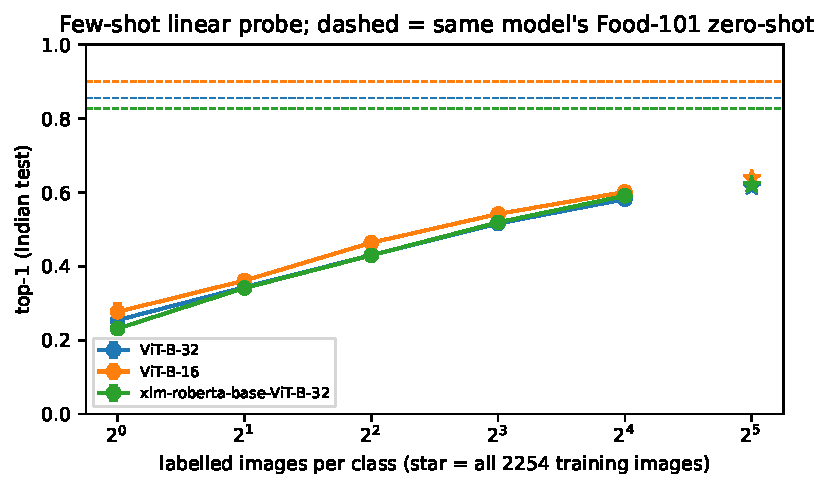
\includegraphics[width=0.8\linewidth]{fewshot_curve.pdf}
% \caption{Few-shot linear probe accuracy on the Indian test set.}\label{fig:fewshot}
% \end{figure}

\section{Discussion and Limitations}
% Noisy scraped labels, small test set (15/class), Food-101 overlap, Hindi spellings, compute limits.
\todo{discussion}

\section{Conclusion}               % Owner: WP4
\todo{conclusion}

\section*{Code availability}
\todo{GitHub URL}

\bibliographystyle{plain}
\bibliography{refs}
\end{document}
